
\documentclass[preprint,12pt]{elsarticle}

\usepackage[spanish]{babel}
\usepackage{amssymb}
\usepackage{graphicx}
\usepackage{lineno}
\usepackage[utf8]{inputenc}
\usepackage{url}
\usepackage{natbib}

\begin{document}
	
	\begin{frontmatter}

		\title{\huge  PROYECTO DE  ANALISIS Y  MEJORAMIENTO DE  SOFTWARE }
		\author{YN Catari Cabrera              (2017059289)\\
		Joaquin Liendo Velásquez (2016054463)
		Piero Limache Victorio ()
		}
		
		\address{Tacna, Perú}
		


%%INICIO abstract
\begin{abstract}
Con el presente documento se pretende presentar de forma concisa y clara las necesidades del cliente en el área a de ventas en términos de software que se realizará. 
En esta documentación se plasmará los requerimientos que servirán de guía para desarrollar el software en sus distintas etapas, ayudándonos a validar e inspeccionar la construcción de este, aplicando la calidad de Software.
Por ello se trabajara con  Sonarqube para el análisis de código estático
para analizar el código y encontrar errores de código, y vulnerabilidades de seguridad. 
El análisis C char de SonarSource tiene una gran cobertura de estándares de calidad bien establecidos.  
\end{abstract}
%%FIN abstract


\end{frontmatter}
%%INICIO Introducción
\section{Antecedentes oIntroducción}

---------------------------------------------------------
%%FIN Introducción

%%INICIO Titulo
\section{Sistema de  Veterinaria Pets}
---------------------------------------------------------
%%FIN Titulo
%%INICIO Autores
\section{Autores}
\begin{itemize}
    \item YN Catari Cabrera
    
    
\end{itemize}
%%FIN Autores
%%INICIO Planteamiento del problema
\section{Planteamiento del problema}
---------------------------------------------------------

%%----------------------------------------------------------------------------------------------------------------------------------------------------------
	\subsection{\textbf{Problema}}
---------------------------------------------------------
%%-----------------------------------------------------------------------------
	\subsection{\textbf{Justificación }}
---------------------------------------------------------

%%-----------------------------------------------------------------------------
	\subsection{\textbf{ Alcance }}
---------------------------------------------------------


\section{Objetivos}
		\subsection{\textbf{ General }}
	 \begin{itemize}
		\item ---------------------------------------------------------
	 \end{itemize}
		\subsection{\textbf{Específicos }}
\begin{itemize}
	\item ---------------------------------------------------------.
	\item --------------------------------------------------------- 
	\item --------------------------------------------------------- 
	\end{itemize}

	\section{Referentes teóricos}
\begin{itemize} 
    \item ---------------------------------------------------------
	\begin{center}
	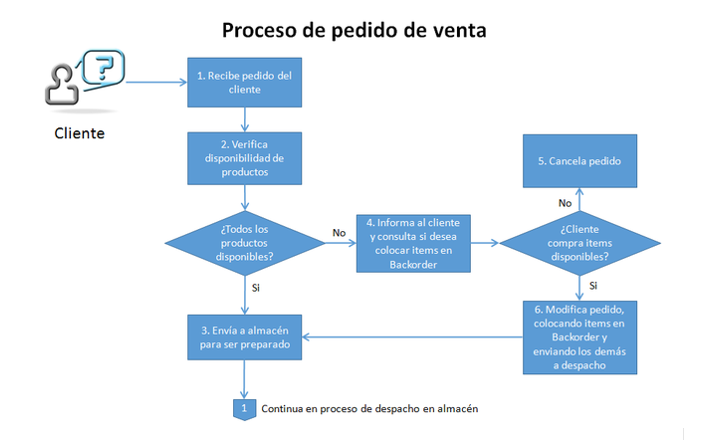
\includegraphics[width=12cm]{./imagen/1} 
	\end{center}
	\item ---------------------------------------------------------

	\item ---------------------------------------------------------

\end{itemize}

\section{Desarrollo de la propuesta}
---------------------------------------------------------
\begin{itemize}
	\item Detección de código duplicado..
	\item Falta de pruebas unitarias, falta de comentarios. 
	\item Código spaghetti, complejidad ciclomática, alto acoplamiento.
	\item Tamaño de archivos de código.
	\item Tamaño de métodos.
	\item No adecuación a estándares y convenciones de código.
	\item Vulnerabilidades conocidas de seguridad.
	
	Una muestra en Nuestro proyecto:
		
    
\end{itemize}

\subsection{\textbf{Tecnología de información  }}
		\begin{itemize}
	\item ---------------------------------------------------------
	\item 	---------------------------------------------------------T.
	\item 	---------------------------------------------------------
	\end{itemize}
\subsection{\textbf{ Metodología, técnicas usadas  }}
---------------------------------------------------------
---------------------------------------------------------
		
\section{Cronograma }

---------------------------------------------------------

\section{Resultado Sonarqube}
	---------------------------------------------------------
	\begin{itemize}
	    \item ---------------------------------------------------------
--------------------------imagen-------------------------------

	
	\end{itemize}
\section{Desarrollo de Solución de Mejora}
\subsection{\textbf{ Casos de Uso de la aplicación}}
----------------------------imagen-----------------------------
\subsection{\textbf{ Diagrama de Arquitectura de la aplicación }}



\begin{itemize}
\item ---------------------------------------------------------
	\item ---------------------------------------------------------
	\item 	---------------------------------------------------------

	\item ---------------------------------------------------------
	\end{itemize}
	---------------------------------------------------------
	---------------------------------------------------------
\subsection{\textbf{ Diagrama de Clases de la aplicación }}
---------------------------------------------------------

\subsection{\textbf{  Metodos de pruebas implementados para coberturar la aplicación }}
\renewcommand{\labelenumi}{{\theenumi})}
\begin{enumerate}

\item ---------------------------------------------------------
\end{enumerate}
\section{Desplegar las pruebas automatizas  Azure Devops y Git gub actions }
---------------------------------------------------------
\begin{itemize} 
    \item ---------------------------------------------------------

\end{itemize}
	\newpage
	
	\bibliography{BIBLIOGRAFIA}	

\end{document}

